%\setcounter{chapter}{1}


%\begin{Large}
%\noindent
%{\bf Lecture 1 \newline
%Dirac Delta Function}
%\end{Large}
%\vspace{1 cm}

\section{Definition of Dirac Delta function and its Representations}
Consider the function $D_{\epsilon}(x)$ defined by
\be
D_{\epsilon}(x) = \left \{ \begin{array}{cl}
                            1/\epsilon & {\rm for}\; -\epsilon/2\leq x \leq \epsilon/2 \\
														0 & {\rm for}\; |x| >\epsilon/2
														\end{array} \right.
														\label{eq:rep1}
\ee														
where $\epsilon$ is a small parameter. The plot of the function is shown below:
\begin{figure}[ht]
\centering
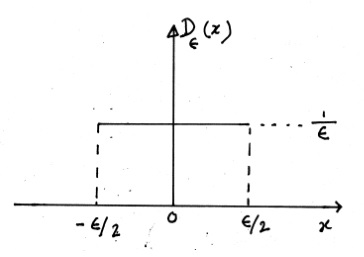
\includegraphics[width=80mm]{rep1.jpg}
\caption{Plot of the function defined in Eq. (\ref{eq:rep1})}
\end{figure}

\noindent
The integral of the function with respect to $x$ is unity, i.e.,
\be
\int_{-\infty}^{\infty} D_{\epsilon}(x) dx =1.
\ee
Now, imagine making $\epsilon$ smaller. As we decrease $\epsilon$, the function gets narrower and taller, but the integral
of the function (i.e., the area under the graph of the function) remains constant at the value 1. In the limit
$\epsilon \rightarrow 0$, the function $D_{\epsilon}(x)$ collapses to a single point, namely $x=0$, and gets infinitely tall. So,
$\lim_{\epsilon\rightarrow 0}D_{\epsilon}(x)$ is not a function at all and the procedure of taking the limit
$\epsilon \rightarrow 0$ is not justified.

\paragraph{}
However, we can make the limiting procedure meaningful if we multiply $D_{\epsilon}(x)$ by some well-defined function
$f(x)$, integrate over $x$ and then take the limit $\epsilon \rightarrow 0$. Consider the integral
\[ \int_{-\infty}^{\infty} D_{\epsilon}(x)f(x)dx \]
where $f(x)$ is a well-defined function. If $\epsilon$ is sufficiently small, the variation of $f(x)$ over the effective
integration interval $[-\epsilon/2,\epsilon/2]$ is negligible and $f(x)$ remains practically equal to $f(0)$. Therefore,
\be
\int_{-\infty}^{\infty} D_{\epsilon}(x)f(x) dx \approx f(0) \int_{-\infty}^{\infty} D_{\epsilon}(x)dx = f(0).
\ee
The smaller the value of $\epsilon$, the better the approximation. In the limit $\epsilon \rightarrow 0$, the above equation is exact:
\be
\lim_{\epsilon \rightarrow 0}\int_{-\infty}^{\infty}D_{\epsilon}(x)f(x)dx = f(0).
\ee
Now, we define the Dirac Delta Function $\delta(x)$ as
\be
\int_{-\infty}^{\infty}\delta(x) f(x)dx \stackrel{{\rm def}}= \lim_{\epsilon \rightarrow 0}\int_{-\infty}^{\infty}D_{\epsilon}(x)f(x)dx = f(0)
\ee
This equation is valid for any function $f(x)$  defined at the origin. More generally, $\delta(x-x_0)$ is defined as
\be
\int_{-\infty}^{\infty} \delta(x-x_0)f(x)dx = f(x_0).
\ee

\paragraph{}
Actually, the integral notation
\[ \int_{-\infty}^{\infty}\delta(x)f(x)dx\]
is not justified because $\delta(x)$ is not really a function. Physically, there is no problem since it becomes impossible to distinguish
between $D_{\epsilon}(x)$ and $\delta(x)$ as soon as $\epsilon$ becomes negligible compared to all distances involved in a physical problem.
Whenever a mathematical difficulty might arise, all we need to do is to assume that $\delta(x)$ is actually $D_{\epsilon}(x)$ with
$\epsilon$ extremely small but not strictly zero.

\paragraph{}
Formally, we can express $\delta(x)$ as a limit of a sequence of proper functions:
\be
\lim_{\epsilon \rightarrow 0}D_{\epsilon}(x) \equiv \delta(x).
\ee
Here $D_{\epsilon}(x)$, which is a proper function of $x$, is called the representation of the delta function. The representation we have discussed so far is the ``square function" given in Eq. (\ref{eq:rep1}). The representation is not unique. There are other functions which 
approach the delta function when appropriate limits are taken.

\subsubsection{\underline{Gaussian Representation}}
Consider the function
\be
D_{\epsilon}(x) =\frac{1}{\epsilon \sqrt{\pi}}e^{-x^2/\epsilon^2} \;\; (\epsilon>0).
\label{eq:rep2}
\ee
For each value of the parameter $\epsilon$, this function satisfies
\be
\int_{-\infty}^{\infty}D_{\epsilon}(x) dx =1.
\ee
This  is the normalized Gaussian function whose plot is shown in the figure below.
\begin{figure}[ht]
\centering
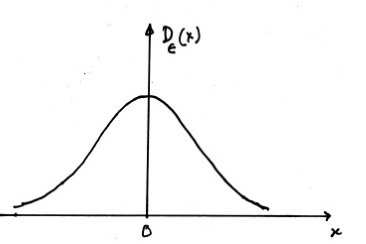
\includegraphics[width=80 mm]{rep2.jpg}
\caption{Plot of the Gaussian function defined in Eq. (\ref{eq:rep2})}
\end{figure}

\noindent
The Gaussian function has a peak at the origin. The peak has a height $1/\epsilon\sqrt{\pi}$ and a width of order $\epsilon$
(exactly how the width is defined doesn't matter). So if $\epsilon$ is allowed to be very small, the peak becomes very tall and very 
narrow. Outside the peak the function becomes extremely small. Thus we have
\be
\delta(x) = \lim_{\epsilon \rightarrow 0} \frac{1}{\epsilon \sqrt{\pi}} e^{-x^2/\epsilon^2}.
\ee

\vspace{10 mm}
\noindent
{\bf Mathematical Notes:} \newline
\noindent
We have the integral
\[ \int_{-\infty}^{\infty}e^{-x^2}dx = \sqrt{\pi}. \]
Now let us consider the following integral
\[ I= \int_{-\infty}^{\infty}e^{-b^2x^2+ a x}dx.\]
First, write
\[ b^2x^2+ax = \left(bx+\frac{a}{2b}\right)^2-\frac{a^2}{4b^2} .\]
Therefore,
\begin{eqnarray*}
I & =& e^{a^2/4b^2}\int_{-\infty}^{\infty}e^{-(bx+a/2b)^2}dx \\
& = & e^{a^2/4b^2}(1/b)\int_{-\infty}^{\infty}e^{-z^2}dz \quad (z=bx+\frac{a}{2b}) \\
& = & e^{a^2/4b^2}\frac{\sqrt{\pi}}{b}.
\end{eqnarray*}

\subsubsection{\underline{Damped Sinusoidal Representation of the Delta Function}}
Consider another function
\be
D_{\epsilon}(x) = \frac{1}{\pi}\, \frac{\sin (x/\epsilon)}{x}\quad (\epsilon > 0).
\label{eq:rep3}
\ee
A plot of the function is shown below.
\begin{figure}[ht]
\centering
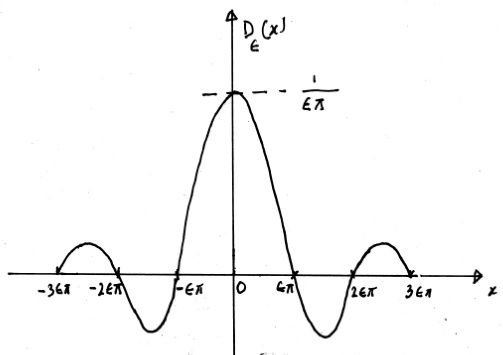
\includegraphics[width=100 mm]{rep3.jpg}
\caption{Plot of the function defined in Eq. (\ref{eq:rep3})}
\end{figure}
The function $D_{\epsilon}(x)$ has the value $1/\epsilon\sqrt{\pi}$ at $x=0$ and it oscillates with decreasing amplitude
as $|x|$ increases. The width of the central maximum is of the order of $\epsilon$ and the period of oscillations with respect to
$x$ is $2\pi \epsilon$.



\noindent
For any value of $\epsilon$ we have
\be
\int_{-\infty}^{\infty} D_{\epsilon}(x)dx = 1.
\ee


\paragraph{}
Thus, the limit of the function as $\epsilon \rightarrow 0$ has all the properties of the delta function: it becomes infinitely large
at $x=0$, and infinitely rapid oscillations as $|x|$ increases means that the entire contribution to an integral containing this
function comes from an infinitesimal neighborhood of $x=0$. We can therefore write
\be
\delta(x) = \lim_{\epsilon \rightarrow 0} \frac{1}{\pi}\, \frac{\sin(x/\epsilon)}{x}
\ee

\vspace{10 mm}
\subsubsection{\underline{Other representation of the Delta Function}}
We can also show that
\begin{eqnarray}
\delta(x) &=& \lim_{\epsilon \rightarrow 0} \frac{1}{2\epsilon}\, e^{-|x|/\epsilon} \\
\delta(x) &=& \lim_{\epsilon \rightarrow 0} \frac{1}{\pi}\, \frac{\epsilon}{x^2+\epsilon^2} \\
\delta(x) &=& \lim_{\epsilon \rightarrow 0} \frac{\epsilon}{\pi}\, \frac{\sin^2(x/\epsilon)}{x^2}.
\end{eqnarray}



\section{Properties of the Delta Function}
It is important to note that, because of its singular character, the $\delta$-function cannot be the end result of a calculation,
and has meaning only so long as a subsequent integral over its argument is carried out. With this understanding we can write
down some relations between delta functions:
\begin{enumerate}
\item
The delta function is an even function, i.e.,
\be
\delta(-x)=\delta(x).
\ee

\item
\be
x\delta(x)=0.
\ee

\item
\be
\delta(ax) = \frac{1}{|a|} \delta(x).
\ee
{\bf Proof:}\newline
Consider the integral
\[
I=\int_{-\infty}^{\infty}\delta(ax)f(x)dx. 
\]
Since the delta function is an even function it doesn't matter if we replace $a$ by $|a|$ in the argument. Thus
\[ I= \int_{-\infty}^{\infty} \delta(|a|x)f(x) dx \, . \]
Making the change of variable
\[ y=|a|x \]
we have
\[ I= \frac{1}{|a|} \int_{-\infty}^{\infty} \delta(y)f(y/|a|) dy= \frac{1}{|a|} f(0) \, , \]
or,
\[ \int_{-\infty}^{\infty} \delta(ax)f(x) dx  = \frac{1}{|a|} \int_{-\infty}^{\infty} \delta(x)f(x) dx \, , \]
i.e.,
\begin{equation*}
\boxed{
\delta(ax)=\frac{1}{|a|}\delta(x)
}
\end{equation*}

\item
More generally, we have
\be
\delta(\phi(x)) = \sum_i \frac{\delta(x-x_i)}{\left|\frac{\partial\phi}{\partial x}\right|_{x_i}}
\ee
where the sum runs over the $x_i$'s which are the simple roots of $\phi(x)$.

\noindent
{\bf Proof:}\newline
Let $x_1, x_2, \cdots , x_N$ be the simple roots of $\phi(x)$ (figure below):
\begin{figure}[ht]
\centering
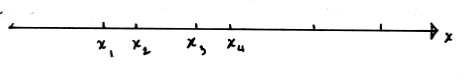
\includegraphics[width=80 mm]{roots.jpg}
\caption{Simple roots of $\phi(x)$.}
\end{figure}

\noindent
In the neighborhood of any of the simple roots $x_i$, we can write
\[ \phi(x) = (x-x_i)\psi(x) \]
where $\psi(x_i) \neq 0$. We have
\[ \psi(x_i) = \left. \frac{\partial \phi(x)}{\partial x}\right|_{x=x_i}. \]

Now, consider the integral
\begin{eqnarray*}
\int_{-\infty}^{\infty} \delta(\phi(x))f(x)dx &=& \sum_{i=1}^N\int_{x_i-\epsilon}^{x_i+\epsilon}
\delta\left[(x-x_i)\psi(x_i)\right]f(x)dx \\
& = & \sum_{i=1}^N  \frac{1}{|\psi(x_i)|}  \int_{x_i-\epsilon}^{x_i+\epsilon} \delta(x-x_i)f(x)dx \\
& = & \sum_{i=1}^N\frac{1}{|\frac{\partial \phi}{\partial x}|_{x=x_i}}  \int_{-\infty}^{\infty} \delta(x-x_i)f(x)dx \\
& = & \sum_{i=1}^N\frac{1}{|\frac{\partial \phi}{\partial x}|_{x=x_i}}  f(x_i) 
\end{eqnarray*}
The above result is obtained if we write
\be
\delta(\phi(x)) = \sum_{i=1}^N \frac{\delta(x-x_i)}{~~\left| \frac{\partial \phi}{\partial x} \right|_{x=x_i} }. \quad {\rm Proved.}
\ee

\item
A frequently used example of the above result is
\be
\delta(x^2-a^2) = \frac{1}{2a}\delta(x-a) + \frac{1}{2a}\delta(x+a), \;\;\; (a>0).
\ee
Here
\[ \phi(x) = x^2-a^2 = (x-a)(x+a). \]
The two simple roots of $\phi(x)$ are at $x=a$ and $x=-a$. Now
\[ \left| \frac{\partial \phi}{\partial x}\right|_{x=a} = |2x|_{x=a} = 2a \]
and
\[ \left| \frac{\partial \phi}{\partial x}\right|_{x=-a} = |2x|_{x=-a} = 2a .\]
Therefore, the above result follows.

\item
\[ f(x)\delta(x-a) = f(a)\delta(x-a).\]

\item
\[ \int \delta(x-y)\delta(y-a) dy = \delta(x-a). \]

\end{enumerate}

\noindent
{\bf Note 1:}\newline
We have the identity
\[ x\delta(x) = 0. \]
The converse is also true and it can be shown that the equation
\[ xu(x)=0 \]
has the general solution
\[ u(x) = c \delta(x).\]

\vspace{10 mm}
\noindent {\bf Note 2:}\newline
We will now prove an identity which is particularly useful in quantum mechanics:
\be
\lim_{\epsilon \rightarrow 0^+} \int_{-\infty}^{\infty} \frac{1}{x \pm  i\epsilon}\, f(x)dx =
\mathcal{P} \int_{-\infty}^{\infty}\frac{dx}{x} f(x)  \mp i\pi f(0),
\ee
or, in short 
\be
\lim_{\epsilon \rightarrow 0^+} \frac{1}{x\pm i\epsilon} = \mathcal{P} \left( \frac{1}{x} \right) \mp i\pi \delta(x),
\ee
where it is understood that the second of these two equations have meaning only within an integral. The symbol $\mathcal{P}$
means the the principal part of an integral where the integrand has a simple pole. The principal part is defined as
\be
\mathcal{P} \int_{-A}^{B} \frac{dx}{x} f(x) = \lim_{\eta \rightarrow 0^+}\left[ \int_{-A}^{-\eta} + \int_{\eta}^B\right]
\frac{dx}{x} f(x).
\ee

\noindent
{\bf Proof:}\newline
We can write
\be
\frac{1}{x\pm i\epsilon} = \frac{x\mp i\epsilon}{x^2+\epsilon^2}= \frac{x}{x^2+\epsilon^2} \mp \frac{i\epsilon}{x^2+a^2}.
\label{eq:pv1}
\ee
Now, we have
\[ \lim_{\epsilon \rightarrow 0^+} \frac{1}{\pi}\, \frac{\epsilon}{x^2+ \epsilon^2} = \delta(x). \]
Therefore,
\be
\lim_{\epsilon \rightarrow 0^+} (\mp) i \frac{\epsilon}{x^2+a^2} = \mp i\pi \delta(x).
\ee
Next, consider the first term on the right and side of Eq. (\ref{eq:pv1}). We multiply this term by a function $f(x)$ which is regular 
at the origin and then integrate over $x$. We get

\begin{multline}
\lim_{\epsilon \rightarrow 0^+} \int_{-\infty}^{\infty}\frac{xf(x)}{x^2+a^2} dx \\
= \lim_{\epsilon \rightarrow 0^+} \left[ \lim_{\eta \rightarrow 0^+} \int_{-\infty}^{-\eta}\frac{xf(x)}{x^2+a^2} dx 
+ \lim_{\eta \rightarrow 0^+} \int_{-\eta}^{\eta}\frac{xf(x)}{x^2+a^2} dx 
+ \lim_{\eta \rightarrow 0^+} \int_{\eta}^{\infty}\frac{xf(x)}{x^2+a^2} dx \right]
\label{eq:pv2}
\end{multline}
Note that we take the limit over $\eta$ first and the we take the limit over $\eta$. Now consider the second integral of the above equation.
\[
\lim_{\eta \rightarrow 0^+} \int_{-\eta}^{\eta}\frac{xf(x)}{x^2+a^2} dx= f(0) \lim_{~\eta \rightarrow 0^+}
\frac{1}{2} \left[ \ln (x^2+ \epsilon^2) \right]_{x=-\eta}^{x=\eta} = 0.
\]
If we now reverse the order of the evaluation of limits in Eq. (\ref{eq:pv2}), the $\epsilon \rightarrow 0^+$ limit
causes no difficulties in the other two integrals. We thus have
\begin{eqnarray*}
\lim_{\epsilon \rightarrow 0^+} \int_{-\infty}^{\infty}\frac{xdx}{x^2+a^2}f(x) &=& \lim_{\eta \rightarrow 0^+}
\lim_{\epsilon \rightarrow 0^+}\left[ \int_{-\infty}^{-\eta} + \int_{\eta}^{\infty}\right] \frac{xdx}{x^2+a^2}f(x) \\
&=& \lim_{\eta \rightarrow 0^+} \left[ \int_{-\infty}^{-\eta} + \int_{\eta}^{\infty}\right] \frac{dx}{x}f(x)\\
&=& \mathcal{P}  \int_{-\infty}^{\infty} \frac{1}{x} f(x)dx
\end{eqnarray*}
This establishes the identity.


\section{Derivative of the Delta Function}
One may define the derivative $\delta^{\prime}(x)$ of the delta function. When $\epsilon$ is small, the derivative of 
$D_{\epsilon}(x)$ has two peaks close to the origin, one peak being positive and the other negative as shown in the figure
below.
\begin{figure}[ht]
\centering
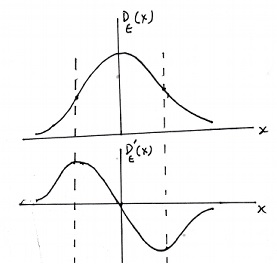
\includegraphics[width=90 mm]{derivative.jpg}
\caption{Plot of $D_{\epsilon}(x)$ and $D^{\prime}_{\epsilon}(x)$.}
\end{figure}


\noindent
As $\epsilon \rightarrow 0$, each of the peaks become very narrow and very tall, and each of the two peaks approach very close to the
origin.  Now, an integration by parts gives
\be
\int_{-\infty}^{\infty} D_{\epsilon}^{\prime}(x)f(x) dx = \left[ D_{\epsilon}(x)f(x)\right]_{-\infty}^{\infty}
- \int_{-\infty}^{\infty} D_{\epsilon}(x) f^{\prime}(x) dx\, . 
\ee
Because $D_{\epsilon}(x)$ tends to zero as $x \rightarrow \pm \infty$, the first term on the right hand side vanishes unless
$f(x)$ explodes violently at infinity. So by letting $\epsilon \rightarrow 0$, we arrive at the definition of
$\delta^{\prime}(x)$:
\be
\boxed{
\int_{-\infty}^{\infty} \delta^{\prime}(x) f(x) dx = - \int_{-\infty}^{\infty}\delta(x)f^{\prime}(x) dx = -f^{\prime}(0).
}
\label{eq:deltaprime}
\ee
From this we immediately get 
\be
\boxed{
x\delta^{\prime}(x) =-\delta(x).
}
\ee
Conversely, it can be shown that the general solution of the equation
\[ xu(x) = \delta(x) \]
can be written as
\[ u(x) =-\delta^{\prime}(x) + c \delta(x) \]
where the second term arises from the homogeneous equation
\[ x\delta(x) = 0. \]
From the definition (\ref{eq:deltaprime}) it also follows that
\be
\boxed{
\delta^{\prime}(-x) = - \delta^{\prime}(x).
}
\ee
The $n^{th}$ order derivative of $\delta(x)$ can be defined in the same way. We find
\be
\int_{-\infty}^{\infty} \delta^{(n)}(x) f(x) dx = (-1)^n f^{(n)}(0).
\ee
We can also prove the following properties of the derivatives of the delta function:
\begin{eqnarray*}
\delta^{(m)}(x)& = &(-1)^m \delta^{(m)}(-x)  \\
x^{m+1}\delta^{(m)}(x)& = & 0  \\
x \delta^{(m)}(x)& = &-(m-1) \delta^{(m-1)}(x).
\end{eqnarray*}


\section{Integration of the Delta Function}
Consider the indefinite integral
\be
\theta_{\epsilon}(x) = \int_{-\infty}^x D_{\epsilon}(y)dy .
\label{eq:theta}
\ee
A graph of $\theta_{\epsilon}(x)$ versus $x$ is shown below.
\begin{figure}[ht]
\centering
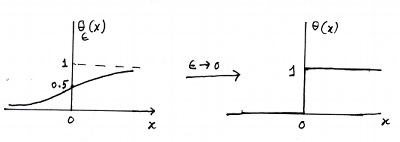
\includegraphics[width=\linewidth]{theta.jpg}
\caption{The $\theta$-function as an integral of the delta function}
\end{figure}


\noindent
As $\epsilon \rightarrow 0$, the step in the function $\theta_{\epsilon}(x)$ gets progressively steeper, until, finally, the function changes abruptly from 0 to 1 at $x=0$. Therefore, taking the limit $\epsilon \rightarrow 0$ in Eq. (\ref{eq:theta})
we have
\be
\theta(x) = \int_{-\infty}^x\delta(y)dy
\label{eq:theta2}
\ee
where
\be
\theta(x) = \left\{ \begin{array}{cl}
                     1 & {\rm for}\; x>0 \\
										0 & {\rm for}\; x<0.
										\end{array} \right.
\ee										
If we differentiate Eq. (\ref{eq:theta2}) with respect to $x$, we get
\be
\frac{d\theta(x)}{dx} = \delta(x).
\ee


\section{Three dimensional delta function}
The three-dimensional delta function $\delta(\vec{r}\,)$ is defined as
\be
\delta(\vec{r}\,) \stackrel{{\rm def}} \equiv \delta(x) \delta(y) \delta(z).
\ee
In other words, $\delta(\vec{r}\,)$ is zero if any of the coordinates $x$, $y$ and $z$ is {\underline{not}} equal to 
zero and $\delta(\vec{r}\,)$ tends to infinity at the origin, i.e., when $x=0$, $y=0$ and $z=0$, such that
\be
\int_{{\rm volume}}\delta(\vec{r}\,)d^3r = 1
\ee
if the volume of integration contains the origin. We also have
 \be
\int \delta(\vec{r}\,)f(\vec{r}\,)d^3r = f(0)
\ee
where again the volume of integration contains the origin. 

\vspace{10 mm}
\noindent
{\bf Note:}
\begin{itemize}
\item
$\delta(\vec{r} - \vec{r}^{\;\prime}\, ) = \delta(x-x^{\prime})\delta(y-y^{\prime})\delta(z-z^{\prime})$
\item $ \int_{V} \delta(\vec{r} - \vec{r}^{\;\prime}\, )d^3r =1 $
\newline
where the volume of integration includes the point $\vec{r}^{\;\prime}$. Otherwise, the integral is zero.
\item $ \int_{V} \delta(\vec{r} - \vec{r}^{\;\prime}\, ) f(\vec{r}\,)d^3r = f(\vec{r}^{\; \prime})$ \newline
if $V$ includes the point $\vec{r}^{\;\prime}$.

\end{itemize}



\subsubsection{A useful formula}
Consider the integral
\begin{eqnarray*}
\int_{-\infty}^{\infty}e^{ikx} dx &=& \lim_{L\rightarrow \infty} \int_{-L}^{L} e^{ikx}dx \\
&=& \lim_{L\rightarrow \infty} \frac{1}{ik}\, \left(e^{ikL}-e^{-ikL} \right) \\
&=& \lim_{L\rightarrow \infty} \, \frac{2}{k} \left( \frac{ e^{ikL}-e^{-ikL}}{2i} \right) \\
&=& \lim_{L\rightarrow \infty}\, \frac{2}{k}\sin kL \\
&=& 2\pi \lim_{L\rightarrow \infty}\, \frac{\sin kL}{\pi k}\\
&=& 2\pi \delta(k),
\end{eqnarray*}
where we have used
\be
\lim_{\epsilon \rightarrow 0} \frac{ \sin (x/\epsilon)}{\pi x} = \delta(x).
\ee
Thus, we have the very important formula
\be
\boxed{
\int_{-\infty}^{\infty}e^{ikx}dx = 2\pi \delta(k)
}
\label{eq:ft3}
\ee
In Eq. (\ref{eq:ft3}) if we integrate with respect to $k$, we would have $\delta(x)$ on the right hand side,
\be
\boxed{
\int_{-\infty}^{\infty}e^{ikx}dk = 2\pi \delta(x)
}
\label{eq:ft4}
\ee
Also note that in Eq. (\ref{eq:ft3}) we integrate over the full domain of $x$ from $-\infty$ to $\infty$. Making a change of variable $x\rightarrow -x$ does not change the value of the integral. Hence we also have
\be
\boxed{
\int_{-\infty}^{\infty}e^{-ikx}dx = 2\pi \delta(k)
}
\label{eq:ft5}
\ee
Similarly, in Eq. (\ref{eq:ft4}), making the change of variable $k \rightarrow -k$, doesn't change the value of the integral. So we could also write
\be
\boxed{
\int_{-\infty}^{\infty}e^{-ikx}dk = 2\pi \delta(x)
}
\label{eq:ft6}
\ee
Thus, in summary
\be
\int_{-\infty}^{\infty}e^{\pm ikx}dx = 2\pi \delta(k),
\ee
and
\be
\int_{-\infty}^{\infty}e^{\pm ikx}dk = 2\pi \delta(x),
\ee
In three dimensions we have
\be
\int_{{\rm all\; space}}e^{\pm i\vec{k}.\vec{r}}d^3r = (2\pi)^3 \delta(\vec{k}\,).
\ee
\be
\int_{{\rm all\; space}}e^{\pm i(\vec{k}-\vec{k}^{\;\prime}).\vec{r}}d^3r = (2\pi)^3 \delta(\vec{k}-\vec{k}^{\;\prime}\,).
\ee
\be
\int_{{\rm all\; space}}e^{\pm i \vec{k}.(\vec{r}-\vec{r}^{\;\prime})}d^3k = (2\pi)^3 \delta(\vec{r}-\vec{r}^{\;\prime}\,).\ee


\section{Fourier transform}

We can always express a function $f(x)$ in the form
\be
f(x) = \int_{-\infty}^{\infty}e^{ikx}\tilde{f}(k)dk
\label{eq:ft10}
\ee
where $\tilde{f}(k)$ is a function of $k$, called the Fourier transform of $f(x)$. From Eq. (\ref{eq:ft10}) we can write
\begin{eqnarray*}
\int_{-\infty}^{\infty}e^{-ik^{\prime}x}f(x)dx &=& \int_{-\infty}^{\infty}\int_{-\infty}^{\infty}e^{i(k-k^{\prime}\,)x}
\tilde{f}(k)dkdx \\
&=& 2\pi \int_{-\infty}^{\infty}\delta(k-k^{\prime}\,)\tilde{f}(k)dk \\
&=& 2\pi \tilde{f}(k^{\prime}\,)
\end{eqnarray*}
Thus, 
\be
\tilde{f}(k) = \frac{1}{2\pi}\int_{\infty}^{\infty}e^{-ikx}f(x)dx.
\label{eq:ft11}
\ee
The functions $f(x)$ and $\tilde{f}(k)$ are Fourier transform of each other. We can write Eqs. (\ref{eq:ft10}) 
and (\ref{eq:ft11}) in a more symmetrical fashion as follows
\begin{eqnarray}
f(x)& = &\frac{1}{\sqrt{2\pi}} \int_{-\infty}^{\infty}e^{ikx}\tilde{f}(k)dk \\
\tilde{f}(k) &=& \frac{1}{\sqrt{2\pi}}\int_{\infty}^{\infty}e^{-ikx}f(x)dx.
\end{eqnarray}

\paragraph{}
In three dimensions we can write
\be
f(\vec{r}\,) = \frac{1}{(2\pi)^{3/2}} \int e^{i\vec{k}.\vec{r}} \tilde{f}(\vec{k}\,)d^3k.
\ee
Multiplying this equation by $e^{-i\vec{k}^{\; \prime}.\vec{r}}$ and integrating over $\vec{r}$, we have
\begin{eqnarray*}
\int_{{\rm all\; space}} e^{-i\vec{k}^{\; \prime}.\vec{r}} f(\vec{r}\,)d^3r
&=& \frac{1}{(2\pi)^{3/2}} \int d^3r\int d^3k\, e^{i(\vec{k}-\vec{k}^{\; \prime}).\vec{r}}\tilde{f}(\vec{k}\,) \\
&=& \frac{1}{(2\pi)^{3/2}} \int d^3k\, (2\pi)^{3} \delta(\vec{k}-\vec{k}^{\; \prime})\tilde{f}(\vec{k}\,) \\
&=& (2\pi)^{3/2} \tilde{f}(\vec{k}^{\; \prime}\,)
\end{eqnarray*}
Therefore,
\be
\tilde{f}(\vec{k}\,) = \frac{1}{(2\pi)^{3/2}}\int e^{-i\vec{k}.\vec{r}} f(\vec{r}\,)d^3r.
\ee


\noindent
In summary, 

\begin{eqnarray}
f(\vec{r}\,)& =& \frac{1}{(2\pi)^{3/2}} \int e^{i\vec{k}.\vec{r}} \tilde{f}(\vec{k}\,)d^3k, \\
\tilde{f}(\vec{k}\,)& =& \frac{1}{(2\pi)^{3/2}}\int e^{-i\vec{k}.\vec{r}} f(\vec{r}\,)d^3r.
\end{eqnarray}


\newpage

\subsection{Parseval Identity}
We will now prove the important identity
\be
\int \left|f(\vec{r}\,)\right|^2d^3r = \int \left| \tilde{f}(\vec{k}\,)\right|^2d^3k.
\ee

\vspace{5 mm}
{\bf \underline{Proof}:}
\begin{multline}
\int \left|f(\vec{r}\,)\right|^2d^3r = \int f(\vec{r}\,) f^*(\vec{r}\,)d^3r \\
=\int d^3r \, \frac{1}{(2\pi)^{3/2}} \int e^{i\vec{k}.\vec{r}} \tilde{f}(\vec{k}\,)d^3k \,
\frac{1}{(2\pi)^{3/2}}   \int e^{-i\vec{k}^{\; \prime}.\vec{r}} \tilde{f}^*(\vec{k}^{\; \prime}\,)d^3k^{\prime}~~~~\\
=\frac{1}{(2\pi)^3}\int d^3k d^3k' \tilde{f}(\vec{k}\,) \tilde{f}^*(\vec{k}^{\; \prime}\,)
\underbrace{ \int d^3r\, e^{i(\vec{k}-\vec{k}^{\; \prime}\,).\vec{r}} }_{(2\pi)^3 \delta(\vec{k}-\vec{k}^{\; \prime}\,) }
\qquad \qquad \qquad ~~~\\
= \int d^3k d^3k' \tilde{f}(\vec{k}\,) \tilde{f}^*(\vec{k}^{\; \prime}\,)\delta(\vec{k}-\vec{k}^{\; \prime}\,) \qquad
\qquad \qquad \qquad \qquad ~~~~~~\\
= \int d^3k  \tilde{f}(\vec{k}\,) \tilde{f}^*(\vec{k}\,) \qquad \qquad \qquad \qquad \qquad\qquad\qquad\qquad
~~~~~ \\
= \int d^3k \left | \tilde{f}(\vec{k}\,) \right|^2. \qquad \qquad \qquad \qquad \qquad \qquad \qquad \qquad \qquad ~~
\end{multline}

The proof is now complete.


					




